\chapter{Accounting for the vectorial nature of light propagation in holographic microscopy}
\label{ch:debye}



%Infinity corrected objectives enable a robust range of placements for the
%tube lens relative to the back aperture of the objective without noticeable
%loss in image quality. 

\section{Introduction}

The model for image formation outlined in \autoref{ch:hvm} provides a full
vectorial treatment of the propagation of the illuminating plane wave and
the resulting scattered fields up to the focal plane of the objective lens.
From there, the model assumes implicitly that the objective and tube lens
simply magnify and relay the intensity pattern to the
camera plane.
This is a fundamental assumption of traditional microscopy and is justified
by a century of optical engineering devoted to minimizing aberrations.
These optical systems are, however, optimized for incoherent imaging of specimens located in the focal plane.
This chapter assesses how well the linear magnification assumption works for
coherent imaging of scatters far from the focal plane. To do this, we will
account for the propagation of the light's electric field from
the specimen plane to the imaging plane. Our model includes the
refraction, reflection, lateral magnification, and angular demagnification
of the fields as they propagate through the objective lens and tube lens
before arriving at the camera plane. We will attempt a full vectorial
treatment throughout and will validate any scalar wave approximations
made along the way. Our approach parallels and extends the work of
Ovyrn and Izen\cite{izen00} and the work of \c{C}apo\u{g}lu \emph{et al.}
\cite{capoglu12}. In particular, we follow the approach of the
former and adopt the mathematical conventions and machinery of the latter.
Our work justifies the use of the scalar theory presented in \autoref{ch:hvm} and
probes the physical limits of HVM set by collecting, refocusing, and recording
the superposition of the incident beam and scattered wave.

\begin{figure}
  \centering
  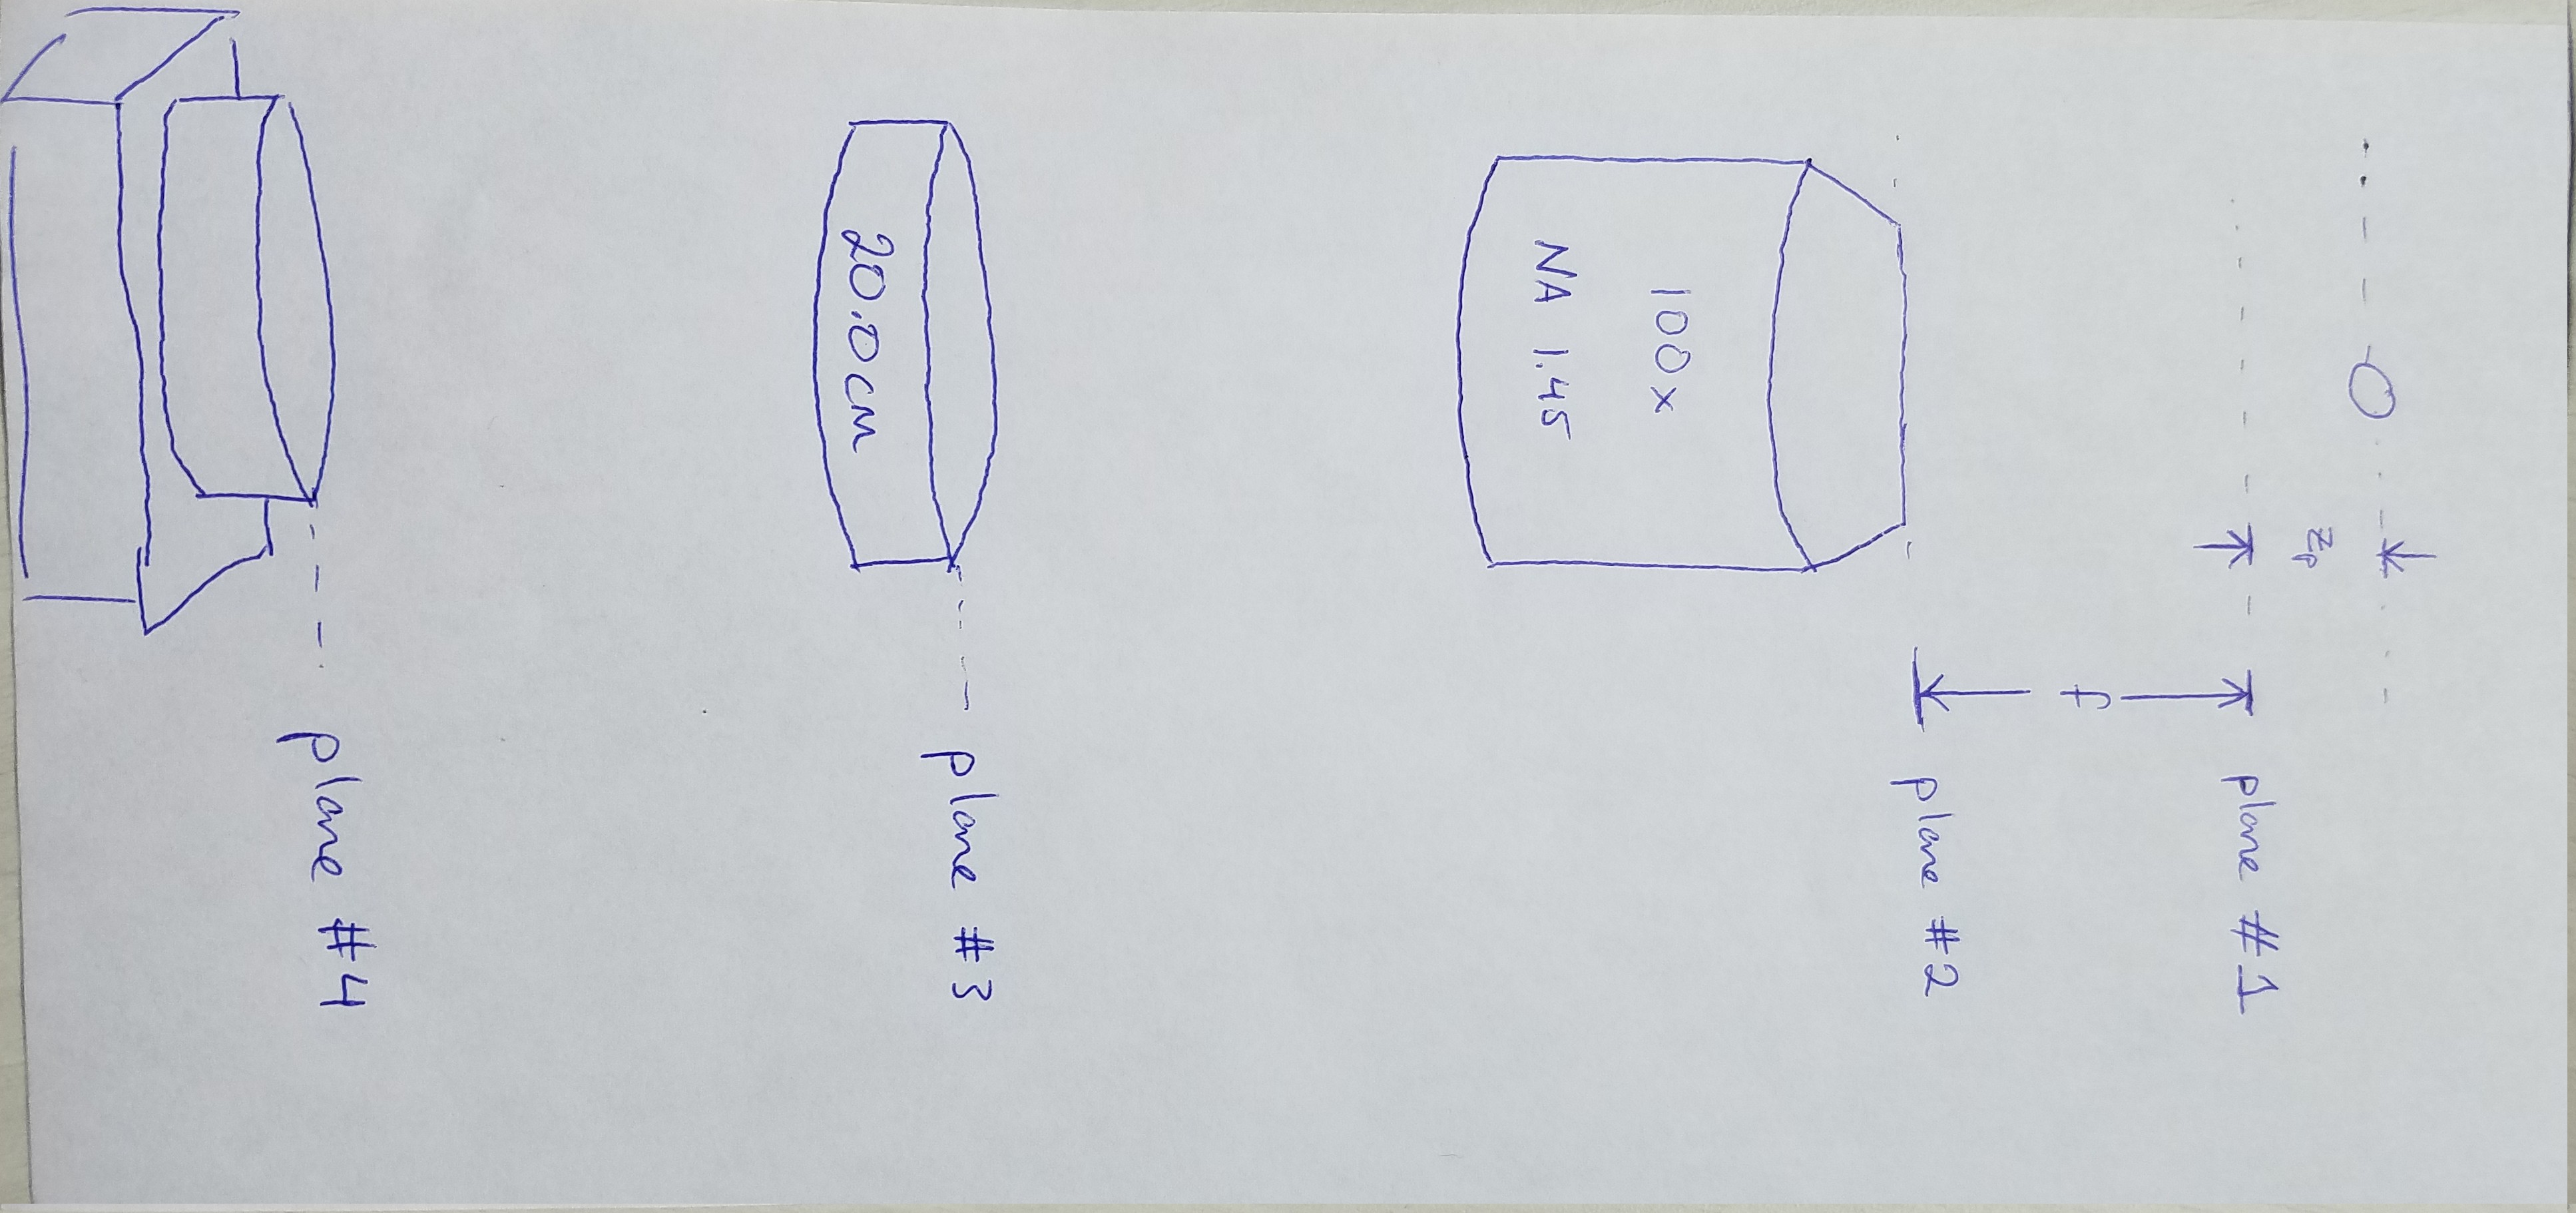
\includegraphics[angle=90,origin=c,width=0.5\textwidth]{debye_wolf_schematic}
  \caption{Diagram depicting the planes at which the fields are evaluated.
    (a) The fields propagate through the focal plane (plane 1) of the objective.
    (b) The fields collected by the objective's entrance pupil (plane 2).
    (c) The fields are focused by the tube lens (plane 3) and arrive at the
    imaging plane (plane 4) of the camera.}
  \label{fig:debye_schematic}
\end{figure}

\section{Modeling the optical train}

With the exception of a coherent illumination source, our holographic microscope
can be reduced to the four essential components of a conventional microscope:
the sample, an objective, a tube lens, and a camera. In the previous chapter,
we described the scattering of a plane wave by a spherical scatterer up to
the focal plane of the objective. We will now evaluate the scattered field and
the plane wave at several interfaces as they propagate along the optical axis
to the camera plane. Figure \ref{fig:debye_schematic} illustrates the four planes
of interest. In the proceeding sections, we will perform the following calculations
for the scattered field:
\begin{enumerate}
\item Evaluate the electric field strength factor for the scattered field at
  the entrance pupil of the objective.
\item Account for the axial displacement of the particle away from the focal
  plane of the objective.
\item Compute the electric field strength factor at the exit of the tube lens
  by accounting for the angular demagnification imposed by the objective.
\item Use a near-field-to-far-field transform to determine the scattered
  fields at the imaging plane of the camera.
\end{enumerate}
The linearity of our optical system allows us to consider the incident field
and scattered field separately. We will derive the transformations for the
scattered field first and then summarize the resulting transformation for the
plane wave.

\subsection{Scattering to the entrance pupil}

In \autoref{ch:hvm} we computed the fields resulting from the scattering of
a plane wave by a homogeneous spherical inclusion in an otherwise
homogeneous medium. As depicted in Fig.~\ref{fig:debye_schematic}, we
propagate the radially expanding scattered fields through the focal plane (plane \num{1} in
Fig.~\ref{fig:debye_schematic}) and all the way to the objective's entrance pupil a distance
$z_p + f$ below the particle, where $f$ is the focal length of the objective.
Our objective  (Nikon Plan Apo, $\num{100}\times$, numerical aperture $\num{1.45}$,
oil immersion) was manufactured to have a working distance of $\SI{135}{\um}$.
At this distance, wavelength, and particle size, the scattered field is in the far-zone,
also known as the Fraunhofer zone, given by $z_p + f >> a_p^2/\lambda$. In this
regime, the wave's $r$ dependence approximately takes the following functional form:
\begin{equation}
  \label{eq:strength_factor}
  \vec{E}(r, \theta, \phi) \approx  \vec{E}(\theta, \phi) \frac{e^{ikr}}{r}
\end{equation}
The term $\vec{E}(\theta, \phi)$ is known as the strength factor and
depends only on the polar angle $\theta$ and the azimuthal angle $\phi$. 

Casting the scattered field in terms of its strength factor will simplify
several of the upcoming calculations. Equation~\eqref{eq:strength_factor} however
is only valid when the scattered field is in the far-field regime.
Ovyrn and Izen\cite{izen00} estimate that adopting this approximation induces a maximum
$\SI{2}{\percent}$ error in the calculated intensity in the range of particle
sizes and locations that we consider here. %% FIXME: Check this claim and possible add a reference
% to an appendix that justifies these claims.

\begin{figure}
  \centering
  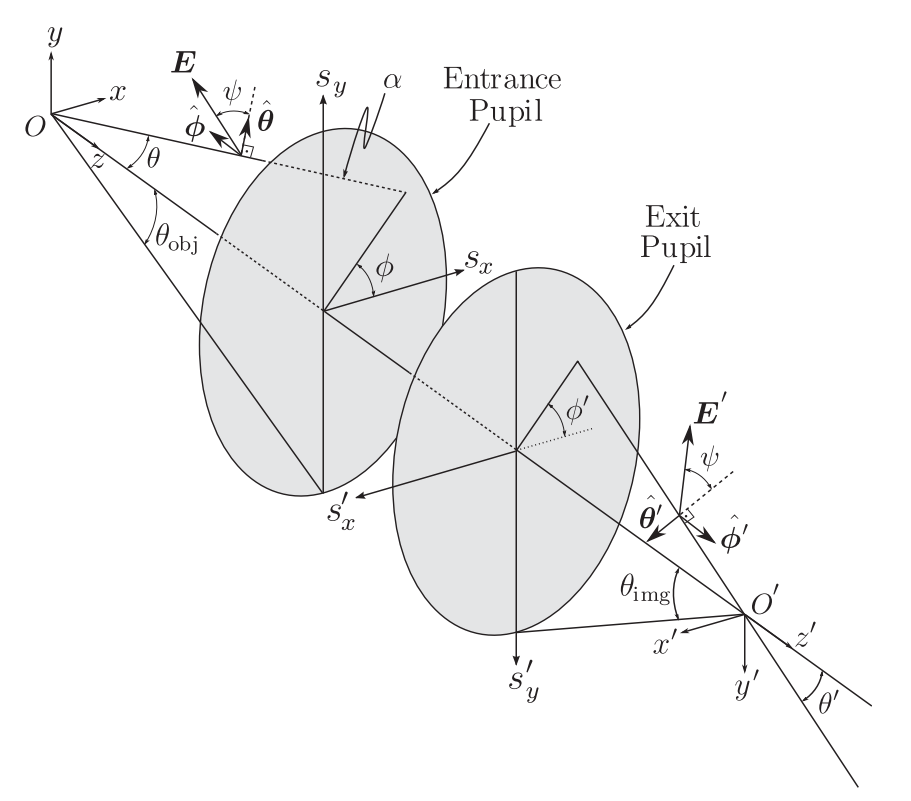
\includegraphics[width=0.75\textwidth]{debye_geom}
  \caption{The two spherical geometries necessary for our description.}
  \label{fig:debye_geom}
\end{figure}

\subsection{ Displacement of the scattered field}

The electric field strength factor $\vec{E}(\theta, \phi)$ is independent
of distance; the fact that the scatterer is a distance $z_p$ away
from the focal plane will be lost in the near-field-to-far-field transform.
As described by Goodman\cite{goodman05},
the scatterer's displacement along the optical axis may be approximated by
a relative phase shift of the electric field strength factor
\footnote{In Goodman's text\cite{goodman05}, this would be a negative
  distance and yet in our geometry we have defined it to be a positive distance.
  Therefore we adopt Eq. 3-66 of Goodman with the alteration that  $z \rightarrow -z$.}
\begin{equation}
  \label{eq:entrance_pupil}
    \vec{E}(\theta, \phi)|_{\text{scatter plane}} \approx \vec{E}(\theta, \phi)|_{\text{focal plane}} e^{-i\frac{2\pi}{\lambda}z\cos{\theta} }.
  \end{equation}

%The scattered field above gives an electric field strength factor that
%emanates from the origin of its coordinate system. In the eyes of the
%collection step, this will mean that the scatterer is located at the origin
%of the focal plane. The scatterers we hope to investigate will be staged 
%some distance z above the focal plane such that the interefence patterns 
%culiminating in the camera plane will be maximally-information dense.

%Note, we will later adopt the direction cosines $(s_x, s_y)$ used in

\subsection{Collection}
In its transit through the optical train from plane \#1 to the camera plane \#4, 
the scattered field experiences an angular demagnification 
that imparts a scaling, polarization rotation, and lensing effect.
In total this effect can be accounted for by
a coordinate transformation governed by the Abbe Sine condition and by scaling
each ray to obey the conservation of energy.

The Abbe Sine condition 
\begin{equation}
  M = \frac{n_m \sin \, \theta}{n^{\prime} \sin \, \theta^{\prime}}
  \label{eq:abbe_sine}
\end{equation}
is necessary for sharp imaging \cite{capoglu12} and is rigorously obeyed by modern optics.
Here, $M$ is the system's lateral magnification, $n_m$ is the medium's refractive index,
and $n'$ is the refractive index of air the camera.
A ray entering the objective at angle $\theta$ relative to the optical axis exits
the tube lens at an angle $\theta^{\prime}$ with a polarization rotation of
$\SI{180}{\degree}$ to the ray as portrayed in Fig.~\ref{fig:debye_geom}.
Additionally, angular demagnification concentrates the electromagnetic radiation
to a smaller solid angle and increases the magnitude of the electric field strength
factor. Accounting for these three effects, we relate the field strength at the
entrance pupil of the objective to the field strength at the tube lens as
  \begin{equation}
    \begin{split}
    \vec{E}'(\theta', \phi')\cdot\hat{\theta'} & = - M \sqrt{ \frac{n'\cos{\theta'}}{n\cos{\theta}}}\vec{E}(\theta, \phi)\cdot\hat{\theta} \hspace{0.2 in}\text{and}\\
    \vec{E}'(\theta', \phi')\cdot\hat{\phi'} & = - M \sqrt{ \frac{n'\cos{\theta'}}{n\cos{\theta}}}\vec{E}(\theta, \phi)\cdot\hat{\phi}.
    \end{split}
  \end{equation}

\subsection{Refocusing the fields to the camera plane}
Finally we utilize a near-field-to-far-field transform to propagate the scattered
field from the tube lens to the imaging plane.
The Debye-Wolf diffraction integral transforms the electric field strength factor at a lens
surface to the electric fields present in the focal plane of that lens.
\begin{equation}
  \vec{E}_{img}(x', y') = \frac{i k'}{2 \pi} \iint_{\Omega_{img}} \vec{E}_s'(s'_x, s'_y) e^{-ik'(s'_xx'+s'_yy')}\frac{ds'_xds'_y}{\cos{\theta'}}
\end{equation}
This integral acts as an inverse of Huygen's principle; a spherical wave is
decomposed into a multitude of plane waves whose phase relations and subsequent
interference produce the same effect as the original spherical wave.
The imperfections present in the optical train are beyond the scope
of this study, however, the Debye-Wolf integral can easily account for a phase
aberration  $\Phi(s'_x,s'_y)$ of the field as it passes through the optical train.
To do so, the integrand of the Debye-Wolf integral is multiplied by a phase term
$e^{ik'\Phi(s'_x,s'_y)}$.

%Several points are worth mentioning:
%\begin{enumerate}
%\item The Debye Wolf integral takes a field strength factor $\vec{E}_s'$,
%  an integration domain $\Omega_{img}$ and the wavenumber $k'$ as its inputs.
%  From these inputs, the electric field in the (x'-y') plane is
%  calculated. 
%\item Heuristically, one should imagine that $\Omega_{img}$ dictates how far 
%  away the plane $(x'-y')$ will be (the distance scales with the size of 
%  $\Omega_{img}$), that $k'$ gives the field strength factor the necessary 
%  units to become an electric field and the electric field strength factor 
%  contains most of the information detailing the interference pattern in the
%  x'-y' plane ($k'$ has influence here as well).
%\item This integral in many ways amounts to
%  an inverse of Huygen's rule; a spherical wave is decomposed into a multitude 
%  of plane waves whose phase relations and subsequent inteference produce
%  the same effect as the original spherical wave.
%\item The Debye-Wolf formalism easily accounts for any phase aberration 
%  $\Phi(s'_x,s'_y)$ of the field as it passes through the optical train. To do so, the integrand
%  of the Debye-Wolf integral is multiplied by a phase term $e^{ik'\Phi(s'_x,s'_y)}$.
%\end{enumerate}

With the exception of the $k'$ in the phase term and the $\cos{\theta'}$ 
modifying the differential element, we should recognize the
Debye-Wolf integral as a Fourier transform. We will discretize this
Fourier transform subject to sampling and aliasing conditions described
in the appendix \ref{app:discretize_dw}. Here we summarize and interpret the result
\begin{equation}
  \begin{split}
    \vec{E}_{img}( m \Delta_x, n \Delta_y) & \approx \frac{i k' \Delta s'_x \Delta s'_y}{2 \pi} e^{-i2\pi \left ( \frac{s'_{x_o}}{\Delta s'_x N_p} m + \frac{s'_{y_o}}{\Delta s'_yN_q} n \right ) } \vec{E}\left [ m, n \right ] \\
    \vec{E}\left [ m,n \right ] & = \sum_{p=0}^{N_p-1}\sum_{q=0}^{N_p-1}\vec{G'}\left [p,q\right ] e^{-i2\pi \left ( \frac{pm}{N_p}+\frac{qn}{N_q} \right ) } \\
    \vec{G'}(s'_x,s'_y) & \doteq \frac{\vec{E'}_s(s'_x,s'_y)}{\cos{\theta'}}e^{-ik'\Phi(s'_x,s'_y)}
  \end{split}
\end{equation}


\subsection{Propagating the incident field}

The propagation of the incident field through the optical system is easy in
comparison to the scattered field. The incident field 

\begin{enumerate}
\item[1.] Account for the phase displacement on the object side of the objective.
\item[2.] Account for the position independent lateral magnification.
\item[3.] Account for the phase displacement on the image side of the tube lens.
\end{enumerate}

%We will assume the objective lens adequately obeys the Abbe Sine condition.
%In addition, we will trust that the objective obeys the conservation of energy
%for all rays which enter its pupil.
%\begin{enumerate}
%\item[1.] Compute the angular spectrum of the scattered field on a spherical surface
%  in the far-field.
%\item[2.] Apply the apodization caused by the entrance pupil of the objective.
%\item[3.] Account for the direction dependent magnfication. This induces changes in
%  amplitude, phase and direction (thus polarization).
%\item[4.] Compute the electric fields present at the imaging plane from the angular spectru%m in step 3.
%\end{enumerate}


\subsection{Propagating the incident field to the camera plane}
  The reference wave is assumed to be traveling coaxially through the optical
  train. It is collected by the objective, passed through ``infinity'' space
  and then rectified back to a plane wave. In the process, the field is flipped 
  (a $\pi$-shift in phase) but the polarization remains. 
  To maintain the conservation of energy, we should measure the flux of energy 
  a single, infinitesimal patch of the wave as it enters and exits the optical 
  train (see figure 1).

  \begin{eqnarray*}
    I_1 dA_1 &=& I_2 dA_2 \\
    \frac{n_1}{\eta_o} \left | \vec{E}_1 \right |^2 dA_1 &=& \frac{n_2}{\eta_o} \left | \vec{E}_2 \right |^2 dA_2\\
    \frac{n_1}{n_2} \left | \vec{E}_1 \right |^2 \frac{dA_1}{dA_2} &=& \left | \vec{E}_2 \right |^2 \\
    \frac{n_1}{n_2}  \frac{1}{M^2} \left | \vec{E}_1 \right |^2 &=& \left | \vec{E}_2 \right |^2 \hspace{.25 in}\text{magnification by M in -x,-y}\\
  \end{eqnarray*}

  By including the $\pi$-shift, we arrive at a final result for the plane wave:
  \begin{equation}
    \vec{E}_2 = -\frac{1}{M}\sqrt{\frac{n_1}{n_2}} \vec{E}_1     
  \end{equation}

  \subsection{Image in the camera plane}
  
  In this work we have sought to produce an image in the camera plane from the
  fields present in the particle plane. To achieve such a transformation,
  we have treked through the optical train and accounted for various 
  effects including energy conservation, angular demagnification, polarization
  rotation, lensing effects and image formation. In doing so, we've
  implemented the Debye-Wolf formalism via a 2D Fourier transform. To ensure that
  our sampling rate will not cause aliasing, we impose the following condition on
  the sampling number $P$ (the same argument applies to the sampling number $Q$):
  \begin{eqnarray*}
    \Delta s_x &<& \frac{2 \pi}{k W_x} \hspace{.5 in} \text{Eq 142 in Ref.}\\
    \frac{2 \sin{\theta_{img}}}{P} &<& \frac{\lambda}{W_x} \\
    \frac{2 \sin{\theta_{img}}W_x}{\lambda} &<& P \\
    \frac{2 \text{NA}\cdot W_x}{n\lambda} &<& P 
  \end{eqnarray*}
  
  The field $\vec{E}_{img}$ is discretized into a set of points 
  $\left ( \Delta_x, \Delta_y \right )$ in the camera plane. We desire that the
  spacing in the image approximates the real spacing between adjacent 
  pixels of our camera. As such, we seek to satisfy the relation 
  $\Delta_x = M\text{mpp}$. However, this is an integer equation which can only
  be approximately satisfied in general. Pursuing this approximation:
  \begin{eqnarray*}
    \Delta_x &\approx& \text{mpp}\cdot M \\
    \frac{2 \pi}{k' \Delta s_x' N_p} &\approx& \text{mpp}\cdot M \\
    \frac{\lambda'}{N_P} \frac{1}{\Delta s_x'} &\approx& \text{mpp}\cdot M \\
    \frac{\lambda'}{N_P} \frac{P}{2 \sin{\theta_{img}}} &\approx& \text{mpp}\cdot M \\
    \frac{\lambda'}{N_P} \frac{PMn'}{2\text{NA}} &\approx& \text{mpp}\cdot M \\
    \frac{\lambda}{N_P} \frac{P}{2\text{NA}} &\approx& \text{mpp} \\
    \frac{P\lambda}{2\text{NA}\cdot\text{mpp}} &\approx& N_p \\
    \frac{P\lambda}{2\text{NA}\cdot\text{mpp}} &\approx& P+\text{pad}_P \\
    \left ( \frac{\lambda}{2\text{NA}\cdot\text{mpp}} - 1 \right )P &\approx& \text{pad}_P \\    
  \end{eqnarray*}

  \begin{equation}
    \begin{split}
      P > \frac{2 \text{NA}\cdot W_x}{n\lambda} \\
      \text{pad}_P  \approx  \left ( \frac{\lambda}{2\text{NA}\cdot\text{mpp}} - 1 \right )P
    \end{split}
  \end{equation}


  
\section{Comparison to Scalar Diffraction Theory}

Having accounted for the propagation of the incident field and the scattered
field through the optical system, we are now ready to assess the differences
in the vector theory and scalar theory. We will produce a range of synthetic
holograms with the vector-based theory over a range %%FIXME.
We will then fit each synthetic
hologram to the scalar-based theory outlined in \autoref{ch:hvm} to fit each.
The difference between the resulting fit parameters and the known scatterer
properties set a lower bound for the cost of adopting the scalar theory
over the vector-based theory.

\begin{figure}
  \centering
  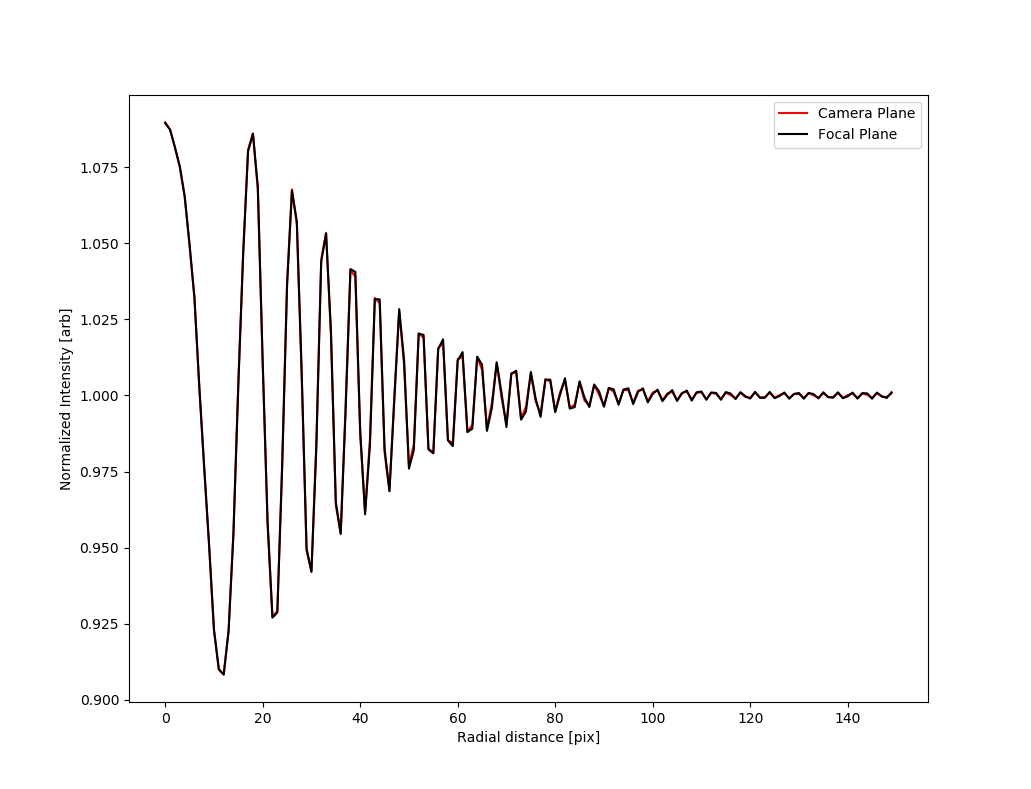
\includegraphics[width=\textwidth]{debye_difference_ps}
  \caption{Comparing the radial profiles of a holographic snapshot taken
    in the focal plane of the objective and the imaging plane of the camera.
    This particular holographic feature is produced by a $\SI{1.0}{\um}$
    diameter polystyrene particle $\SI{13.5}{\um}$ above the focal plane.}
  \label{fig:debye_difference_ps}
\end{figure}


\section{Discussion}

Not much to discuss yet.


